\printnomenclature[3.5cm] % Значение ширины столбца с обозначениями стоит подбирать вручную

\newpage

\begin{figure}[ht]
    \centerfloat{
        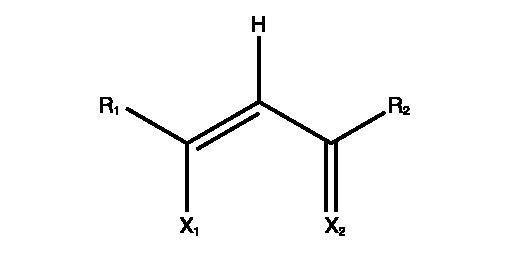
\includegraphics[scale=1.25]{1_stroenie-beta.pdf}
    }
\label{fig:latex}
\end{figure}

\begin{table} [htbp]%
    \centering
    \caption{Исследованные соединения}%
    \label{tab:comopund_list_1}% 
    \renewcommand{\arraystretch}{1.5}%% Увеличение расстояния между рядами, для улучшения восприятия.
    \begin{SingleSpace}
        \begin{tabular}{@{}@{\extracolsep{20pt}}llllll@{}} %Вертикальные полосы не используются принципиально, как и лишние горизонтальные (допускается по ГОСТ 2.105 пункт 4.4.5) % @{} позволяет прижиматься к краям
            \toprule     %%% верхняя линейка
            №         & Compound        & X$_1$      & X$_2$  & R$_1$      & R$_2$      \\
            \midrule 
            I.        & Hmal            & H          & O      & H          & H          \\
            II.       & Hacac           & H          & O      & CH$_3$     & CH$_3$     \\
            III.      & EnAcac          & NH$_2$     & O      & CH$_3$     & CH$_3$     \\
            IV.       & EnMeAcac        & NHCH$_3$   & O      & CH$_3$     & CH$_3$     \\
            V.        & CH$_3$SAcac     & SCH$_3$    & O      & CH$_3$     & CH$_3$     \\
            VI.       & HSHAc           & SH         & O      & CH$_3$     & CH$_3$     \\
            VII.      & SOHAc           & OH         & S      & CH$_3$     & CH$_3$     \\
            VIII.     & HtFAc           & OH         & O      & CF$_3$     & CH$_3$     \\
            IX.       & HhFAc           & OH         & O      & CF$_3$     & CF$_3$     \\
            \bottomrule 
        \end{tabular}
    \end{SingleSpace}
\end{table}

\newpage

\begin{figure}[ht]
    \centerfloat{
        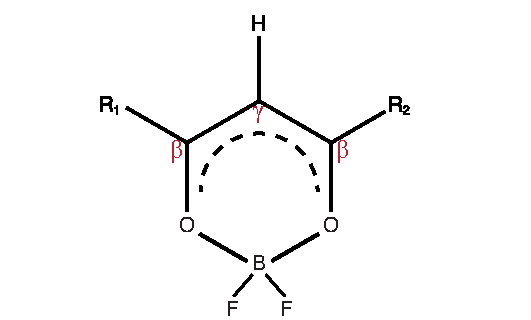
\includegraphics[scale=1.25]{2_stroenie_boron.pdf}
    }
\label{fig:latex}
\end{figure}

\begin{table} [htbp]%
    \centering
    \caption{Исследованные соединения Часть 2}%
    \label{tab:comopund_list_2}% 
    \renewcommand{\arraystretch}{1.5}%% Увеличение расстояния между рядами, для улучшения восприятия.
    \begin{SingleSpace}
        \begin{tabular}{@{}@{\extracolsep{20pt}}llll@{}} %Вертикальные полосы не используются принципиально, как и лишние горизонтальные (допускается по ГОСТ 2.105 пункт 4.4.5) % @{} позволяет прижиматься к краям
            \toprule     %%% верхняя линейка
            №      &Compound         & R$_1$      & R$_2$                           \\
            \midrule
            X.     & BF$_2$Acac      & CH$_3$     & CH$_3$                          \\
            XI.    & BF$_2$bac       & CH$_3$     & C$_6$H$_5$                      \\
            XII.   & BF$_2$tac       & CH$_3$     & 4$-$CH$_3$C$_6$H$_4$            \\
            XIII.  & BF$_2$xac       & CH$_3$     & 2,4$-($CH$_3$)$_2$C$_6$H$_3$    \\
            XIV.   &                 & CH$_3$     & 4$-$biphenyl                    \\
            XV.    &                 & CH$_3$     & 4$-$fluorenyl                   \\
            XVI.   &                 & CH$_3$     & 4$-$trans$-$stilbene            \\
            XVII.  & BF$_2$Dbm       & C$_6$H$_5$ & C$_6$H$_5$                      \\
            XVIII. & BF$_2$anth      & CH$_3$     & C$_{14}$H$_9$                   \\
            XIX.   & BF$_2$naph      & CH$_3$     & C$_{10}$H$_7$                   \\
            XX.    & BF$_2$ben       & CH$_3$     & CO$_2$C$_6$H$_4$                \\
            \bottomrule 
        \end{tabular}
    \end{SingleSpace}
\end{table}